\documentclass[conference]{IEEEtran}
\IEEEoverridecommandlockouts
% The preceding line is only needed to identify funding in the first footnote. If that is unneeded, please comment it out.
\usepackage{cite}
\usepackage{amsmath,amssymb,amsfonts}
\usepackage{ngerman}
\usepackage{algorithmic}
\usepackage{graphicx}
\usepackage{textcomp}
\usepackage{xcolor}
\usepackage{tikz}
\def\BibTeX{{\rm B\kern-.05em{\sc i\kern-.025em b}\kern-.08em
    T\kern-.1667em\lower.7ex\hbox{E}\kern-.125emX}}
\begin{document}

\title{Conference Paper Title*\\
{\footnotesize \textsuperscript{*}Note: Sub-titles are not captured in Xplore and
should not be used}
\thanks{Identify applicable funding agency here. If none, delete this.}
}

\author{
\IEEEauthorblockN{1\textsuperscript{st} Karina Heins}
\IEEEauthorblockA{\textit{DHBW Ravensburg Campus Friedrichshafen} \\
\textit{Mercedes-Benz AG}\\
Friedrichshafen,  Germany \\
heins.karina-tfe18@it.dhbw-ravensburg.de}
\and
\IEEEauthorblockN{2\textsuperscript{st} Florian Schatz}
\IEEEauthorblockA{\textit{DHBW Ravensburg Campus Friedrichshafen} \\
\textit{Mercedes-Benz AG}\\
Friedrichshafen,  Germany \\
schatz.florian-tfe18@it.dhbw-ravensburg.de}
\and
\IEEEauthorblockN{3\textsuperscript{st} Patrick Madlindl}
\IEEEauthorblockA{\textit{DHBW Ravensburg Campus Friedrichshafen} \\
\textit{Mercedes-Benz AG}\\
Friedrichshafen,  Germany \\
madlindl.patri-tfe18@it.dhbw-ravensburg.de}
\and
\IEEEauthorblockN{4\textsuperscript{st} Marcel Dirschinger}
\IEEEauthorblockA{\textit{DHBW Ravensburg Campus Friedrichshafen} \\
\textit{Airbus Helicopters AG}\\
Friedrichshafen,  Germany \\
dirschinger.marcel-tfe18@it.dhbw-ravensburg.de}
}

\maketitle

\begin{abstract}
This document is a model and instructions for \LaTeX.
This and the IEEEtran.cls file define the components of your paper [title, text, heads, etc.]. *CRITICAL: Do Not Use Symbols, Special Characters, Footnotes, 
or Math in Paper Title or Abstract.
\end{abstract}

\begin{IEEEkeywords}
component, formatting, style, styling, insert
\end{IEEEkeywords}

\section{Einleitung}
In der Informatik, aber auch anderen Bereichen,  müssen häufig Daten nach bestimmten Attributen sortiert werden. Liegen diese in digitaler Form vor, kann eine Sortierung der Daten über Sortieralgorithmen gelöst werden.  Bei kleinen Datensätzen ist die Wahl des Sortieralgorithmus aufgrund der geringen Laufzeit nahezu irrelevant.  Steigt die Datensatzgröße verlängert sich dementsprechend die Sortierzeit.  Zur Verkürzung dieser können effiziente Sortierverfahren wie Merge-Sort verwendet werden.  In der heutigen Zeit, in der die Menge der Daten, z. B. Messreihen aus Versuchen, im Verhältnis zur möglichen Rechenleistung eines Computers massiv gestiegen ist, ist eine effiziente Sortierung von hoher Bedeutung. Zur weiteren Optimierung der Sortierung kann Cloud-Computing eingesetzt werden. Dabei werden Rechenaufgaben nicht auf einem einzelnen Computer ausgeführt, sondern können unter Einsatz des Message Passing Interface (MPI) auf mehrere sog. Maschinen verteilt werden. In der Arbeit wird untersucht ob eine Aufteilung der Sotieraufgabe von Wörtern unter EInsatz der BW-Cloud zu einer Verringerung der Laufzeit betragen kann.
\section{Grundlagen}
\subsection{Merge Sort}
\subsection{Merge Sort}
Merge-Sort ist ein effizienter Algorithmus zur Sortierung vergleichbarer Datenobjekte.  Der Algorithmus setzt sich dem Namen nach aus \glqq merge\grqq{} (engl.  für Verschmelzen) und \glqq sort\grqq{} (engl.  für Sortieren) zusammen und wurde 1945 durch John von Neumann vorgestellt. Es handelt sich um einen stabilen Sortieralgorithmus,  der die Reihenfolge zusammengehöriger Eingangsdaten bei eventueller Sortierung über einen weiteren Parameter nicht manipuliert. Außerdem arbeitet der Algorithmus nach dem \glqq Teile und Hersche\grqq{}-Prinzip und setzt dafür folglich auf Rekursion, Merge-Sort wird zum Sortieren und Arrays/Listen bzw.  anderen listenähnlichen Datenstrukturen verwendet.\\
\begin{figure}[htbp]
\centering
% 5-2-3-1-4    10
% 5-2 3-1-4	8.5
% 5 2 3 1-4	7
% 5 2 3 1 4	5.5
% 2-5 3 1-4	4
% 2-5 1-3-4	2.5
%1-2-3-4-5	1
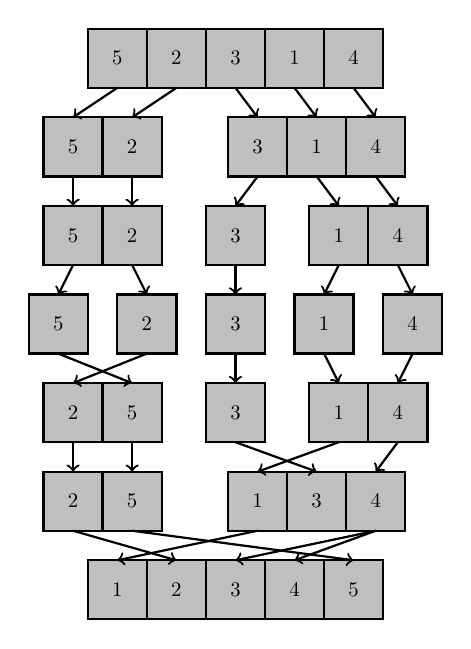
\begin{tikzpicture}[scale=0.75, transform shape]
\draw [thick, fill=gray!50] (1,9) rectangle(2,10) node[pos=.5] {5};
\draw [thick, fill=gray!50] (2,9) rectangle(3,10) node[pos=.5] {2};
\draw [thick, fill=gray!50] (3,9) rectangle(4,10)node[pos=.5] {3};
\draw [thick, fill=gray!50] (4,9) rectangle(5,10)node[pos=.5] {1};
\draw [thick, fill=gray!50] (5,9) rectangle(6,10)node[pos=.5] {4};

\draw [thick, fill=gray!50] (0.25,7.5) rectangle(1.25,8.5)node[pos=.5] {5};
\draw [thick, fill=gray!50] (1.25,7.5) rectangle(2.25,8.5)node[pos=.5] {2};
\draw [thick, fill=gray!50] (3.375,7.5) rectangle(4.375,8.5)node[pos=.5] {3};
\draw [thick, fill=gray!50] (4.375,7.5) rectangle(5.375,8.5)node[pos=.5] {1};
\draw [thick, fill=gray!50] (5.375,7.5) rectangle(6.375,8.5)node[pos=.5] {4};

\draw [thick, fill=gray!50] (0.25,6) rectangle(1.25,7)node[pos=.5] {5};
\draw [thick, fill=gray!50] (1.25,6) rectangle(2.25,7)node[pos=.5] {2};
\draw [thick, fill=gray!50] (3,6) rectangle(4,7)node[pos=.5] {3};
\draw [thick, fill=gray!50] (4.75,6) rectangle(5.75,7)node[pos=.5] {1};
\draw [thick, fill=gray!50] (5.75,6) rectangle(6.75,7)node[pos=.5] {4};

\draw [thick, fill=gray!50] (0,4.5) rectangle(1,5.5)node[pos=.5] {5};
\draw [thick, fill=gray!50] (1.5,4.5) rectangle(2.5,5.5)node[pos=.5] {2};
\draw [thick, fill=gray!50] (3,4.5) rectangle(4,5.5)node[pos=.5] {3};
\draw [thick, fill=gray!50] (4.5,4.5) rectangle(5.5,5.5)node[pos=.5] {1};
\draw [thick, fill=gray!50] (6,4.5) rectangle(7,5.5)node[pos=.5] {4};

\draw [thick, fill=gray!50] (0.25,3) rectangle(1.25,4)node[pos=.5] {2};
\draw [thick, fill=gray!50] (1.25,3) rectangle(2.25,4)node[pos=.5] {5};
\draw [thick, fill=gray!50] (3,3) rectangle(4,4)node[pos=.5] {3};
\draw [thick, fill=gray!50] (4.75,3) rectangle(5.75,4)node[pos=.5] {1};
\draw [thick, fill=gray!50] (5.75,3) rectangle(6.75,4)node[pos=.5] {4};

\draw [thick, fill=gray!50] (0.25,1.5) rectangle(1.25,2.5)node[pos=.5] {2};
\draw [thick, fill=gray!50] (1.25,1.5) rectangle(2.25,2.5)node[pos=.5] {5};
\draw [thick, fill=gray!50] (3.375,1.5) rectangle(4.375,2.5)node[pos=.5] {1};
\draw [thick, fill=gray!50] (4.375,1.5) rectangle(5.375,2.5)node[pos=.5] {3};
\draw [thick, fill=gray!50] (5.375,1.5) rectangle(6.375,2.5)node[pos=.5] {4};

\draw [thick, fill=gray!50] (1,0) rectangle(2,1)node[pos=.5] {1};
\draw [thick, fill=gray!50] (2,0) rectangle(3,1)node[pos=.5] {2};
\draw [thick, fill=gray!50] (3,0) rectangle(4,1)node[pos=.5] {3};
\draw [thick, fill=gray!50] (4,0) rectangle(5,1)node[pos=.5] {4};
\draw [thick, fill=gray!50] (5,0) rectangle(6,1)node[pos=.5] {5};
\draw [thick,draw=black,->] (3.875,1.5) -- (1.5,1);
\draw [thick,draw=black,->] (0.75,1.5) -- (2.5,1);
\draw [thick,draw=black,->] (5.875,1.5) -- (3.5,1);
\draw [thick,draw=black,->] (5.875,1.5) -- (4.5,1);
\draw [thick,draw=black,->] (1.75,1.5) -- (5.5,1);
\draw [thick,draw=black,->] (0.75,3) -- (0.75,2.5);
\draw [thick,draw=black,->] (1.75,3) -- (1.75,2.5);
\draw [thick,draw=black,->] (3.5,3) -- (4.875,2.5);
\draw [thick,draw=black,->] (5.25,3) -- (3.875,2.5);
\draw [thick,draw=black,->] (6.25,3) -- (5.875,2.5);
\draw [thick,draw=black,->] (2,4.5) -- (0.75,4);
\draw [thick,draw=black,->] (0.5,4.5) -- (1.75,4);
\draw [thick,draw=black,->] (3.5,4.5) -- (3.5,4);
\draw [thick,draw=black,->] (5,4.5) -- (5.25,4);
\draw [thick,draw=black,->] (6.5,4.5) -- (6.25,4);
\draw [thick,draw=black,->] (0.75,6) -- (0.5,5.5);
\draw [thick,draw=black,->] (1.75,6) -- (2,5.5);
\draw [thick,draw=black,->] (3.5,6) -- (3.5,5.5);
\draw [thick,draw=black,->] (5.25,6) -- (5,5.5);
\draw [thick,draw=black,->] (6.25,6) -- (6.5,5.5);
\draw [thick,draw=black,->] (0.75,7.5) -- (0.75,7);
\draw [thick,draw=black,->] (1.75,7.5) -- (1.75,7);
\draw [thick,draw=black,->] (3.875,7.5) -- (3.5,7);
\draw [thick,draw=black,->] (4.875,7.5) -- (5.25,7);
\draw [thick,draw=black,->] (5.875,7.5) -- (6.25,7);
\draw [thick,draw=black,->] (1.5,9) -- (0.75,8.5);
\draw [thick,draw=black,->] (2.5,9) -- (1.75,8.5);
\draw [thick,draw=black,->] (3.5,9) -- (3.875,8.5);
\draw [thick,draw=black,->] (4.5,9) -- (4.875,8.5);
\draw [thick,draw=black,->] (5.5,9) -- (5.875,8.5);
\end{tikzpicture}
\caption[Darstellung Merge-Sort Beispiel]{Ablauf eines Merge-Sort über ein Array aus Beispielzahlen}
\label{fig:mergesort}
\end{figure}
Um die Elemente der Datenstruktur (im Folgenden Liste) sortieren zu können,  werden diese zunächst rekursiv geteilt.  Dafür wird die Liste in eine linke und rechte Hälfte geteilt.  Die Hälften stellen jetzt jeweils die Basis für den nächsten Rekursions- bzw- Teilungsschritt dar. Der Vorgang wird wiederholt,  bis pro Teilliste lediglich ein weiters Element vorhanden ist.  Die Teilung der Datenelemente fordert nahezu keine Rechenleistung und benötigt keinen zusätzlichen Speicherplatz.  Im Anschluss wird die Rekursion der Teilung für den eigentlichen Sortiervorgang zurück durchlaufen. Die geteilten Listen werden nun innerhalb der Rekursion zu Zweierpaaren jeweils sortiert in eine neue Liste zusammengeführt. In der Informatik wird dabei auch von Konkatenierung gesprochen.  Aufgrund der Zusammenführung der Listen aus zwei bereits sortierten Teillisten können im Sortiervorgang jeweils die ersten Elemente verglichen werden. Das Element mit dem niedrigeren Wert wird in die Liste der Zusammenführung gespeichert.  Da in diesem Schritt zeitgleich drei Listen vorhanden sind wird hier abseits des ursprünglichen Datenspeichers zusätzlicher Speicher benötigt.  Aufgrund der Vergleiche ergibt sich in der Zusammenführung der überwiegende Rechenaufwand des Algorithmus.  Der Ablauf des \glqq merge\grqq{} bzw. Zusammenführens wird bis zur Startgröße der Liste fortgeführt.\\
Bei Merge-Sort handelt es sich um ein stabiles Sortierverfahren.  Außerdem lässt sich die Laufzeit in der bekannten Landau-Notation darstellen. Im Vergleich zu anderen Sortieralgorithmen beträgt die Laufzeit bei Merge-Sort im schlechtesten,  durschschnittlichen und besten Fall immer:
\begin{math}
\mathcal{O}(n\log n)
\end{math}.
Trotz der immer gleichen Laufzeit nach der Landau-Notation wird in viele Fällen kein Merge-Sort für die Sortierung großer Datenmengen verwendet.  Neben der Betrachtung der Speicherzugriffe muss zudem der zusätzlich benötigte Speicher in die Betrachtung der Laufzeit bzw. Komplexität einbezogen werden.  Wie bereits erwähnt wird beim Zusammenführen der zwei Listen eine dritte Liste benötigt. Diese nimmt im letzten Konkatenierungsschritt die Länge aller Elemente an.  Dementsprechend werden für Merge-Sort neben der Rechenleistung auch ein Speicherbereich in der Größe der Ausgangsdaten benötigt. Trotz der deutlich besseren Komplexität im schlechtesten Fall, werden aufgrund des Speicherbedarfs meist andere Sortierverfahren ohne zusätzlichen Speicherbedarf verwendet.

ggf.:Master-Theorem: 2*T(n/2) + T(n) mit T(x) = n*logn
 \subsection{Message Passing Interface}
%\label{subsection:Message Passing Interface}
Message Passing Interface (MPI) ist ein Standard zum Austausch von Nachrichten zwischen Prozessen auf einem Rechner sowie zwischen Prozessen auf verteilten Rechnern. MPI dient als Programmierschnittstelle und verschickt verpackte Nachrichten an parallel laufende Prozesse.\\
Die Bibliotheken OpenMPI und MPICH setzen den MPI Standard für die Programmiersprache C++ um.
Auf den für das Projekt verwendeten Linux Rechnern steht OpenMPI zur Verfügung und wird für die Paralellisierungsanwendungen des Projektes verwendet.\\ 
\subsubsection{Konzept}
Die Grundidee von MPI besteht aus zwei Konzepten: dem Konzept der Prozessgruppe und dem des Kommunikationskontexts. Diese beiden Begriffe werden im Folgenden erläutert.
\\
Mit Prozessgruppen wird die Anzahl an beteiligten Rechnern definiert. Beim Ausführen des Programms mit MPI werden zu Beginn die beteiligten Prozesse gestartet. Innerhalb des Programms können die einzelnen Prozesse gesteuert und zusätzlich in einzelne Untergruppen zusammengefasst werden.
\\
Einzelne Nachrichten können anhand der Empfänger- bzw. Sender-ID zugeordnet werden. Mit MPI können so Nachrichten zu einem bestimmten Zeitpunkt an einen bestimmten Prozess verschickt werden.\\
Der Kommunikationskontext dient als Lösung bei Überschneidungen der Tag-,Sender- und Empfänger-IDs. Jeder Sende- und Empfangsvorgang gehört zu einem Kontext. Die Kommunikation erfolgt ausschließlich über diesen Kontext, sodass es zu keinen Verwechslungen kommen kann.
Durch einen Kommunikator werden Prozessgruppen und Kommunikationskontexte miteinander vereint. Beim Programmstart wird der allgemeine Kommunikator \textit{MPI\_COMM\_WORLD} erzeugt.~\cite{b1}. Dieser wird auch in diesem Projekt verwendet.\\
\subsubsection{Verwendung} Um MPI zu verwenden muss zunächst MPI initialisiert werden, wobei der oben genannte Kommunikator \textit{MPI\_COMM\_WORLD} erzeugt wird.\\
Mit dem Befehl \textit{MPI\_Comm\_size()} kann die Größe der Gruppe ermittelt werden. Mit dem Befehl \textit{MPI\_Comm\_rank()} kann der Rang der einzelnen Prozesse ermittelt werden. Der Rang beschreibt die Positionen der einzelnen Prozesse innerhalb einer Gruppe.
Die MPI-Laufzeitumgebung kann mit \textit{MPI\_Finalize()} am Programmende gestoppt werden.\\
Zur Punkt-zu-Punkt-Kommunikation über MPI werden die Funktionen \textit{MPI\_Send()} und \textit{MPI\_Recv()} verwendet. Dabei werden einzelne Nachrichten von einem Prozess zu einem anderen verschickt. Diese Art des Sendens ist blockierend. \textit{MPI\_Send()} und \textit{MPI\_Recv()} blockieren das System bis eine Nachricht vollständig verschickt bzw. empfangen wird. Sobald die Nachricht verschickt bzw. empfangen wurde, setzt sich der Programmablauf fort. \\
Ein MPI-basiertes Programm kann mit Eingabe des Befehls \textit{mpirun} sowie einem Verweis auf die zu nutzenden Prozesse bzw. Rechner in einer Konsole gestartet werden. Alle Prozesse, auch wenn diese auf physikalisch anderen Rechnern laufen sollen, werden gleichzeitig gestartet~\cite{b1}.
 \subsection{Cloud Computing}
\section{Umsetzung}
\subsection{Test}
Für das Projekt werden parallel zur Entwicklung der Funktionen Unit Tests mitverfasst. Hierfür verwendet wird die Testsuite \textit{gtest}, welche in \textit{GoogleTest} enthalten ist. Der Zweck der Unit Tests beschränkt sich auf eine Absicherung der Lauffähigkeit und Gewährleistung der Grundfunktionalität des Programms.
\\
Einige Funktionen, welche komplexe Algorithmen enthalten, werden mithilfe von im Vorhinein definierten \textit{Blackbox-Tests} entwickelt. Beispiele sind die Funktionen \textit{split\_even()} und \textit{merge\_back()}. Es werden jeweils ein Standard-Fall und mehrere Randfälle aus verschiedenen Äquivalenzklassen in die Tests aufgenommen. 
Wenn die zu entwickelnden Funktionen diese Tests bestehen, wird angenommen, dass die geforderte Grundfunktionalität erfüllt wird. Robustheit ist nicht gegeben. Eine vollständige Testabdeckung,
wie z.B. die \textit{vollständige Anweisungsüberdeckung} (C0-Überdeckung), wird nicht realisiert.
\\
Auf eine vollständige Testabdeckung nach einer der bekannten Klassen C0...C3 für strukturelle Tests wird generell verzichtet. Gründe hierfür sind die beschränkte Bearbeitungszeit für das Projekt sowie dass eine vollständige Abdeckung nicht zielführend für das Projekt ist. Das Testen von Nutzereingaben im Programm oder der MPI-Funktionalität würde einen hohen Aufwand beim Testentwurf bedeuten. Um die MPI-Funktionalitäten rigoros zu testen, müssten u.a. der Einfluss der Anzahl verwendeter Rechenknoten, die Behandlung von Knoten-Ausfällen sowie die Auswirkungen maximaler Nachrichtenpaketgrößen betrachtet werden. Hiervon wird abgesehen, da die im Rahmen des Projekts entworfene Software nicht produktiv eingesetzt wird und ausschließlich der Übung mit sowie der Demonstration von Vor- und Nachteilen von MPI dient. Die Vorteile einer vollständigen Testabdeckung würden in keinem Verhältnis zum benötigten Aufwand der Testerstellung stehen.
\\
Wäre eine Absicherung der Software durch Tests gewünscht, müssten die eigens entwickelten und implementierten Algorithmen rigoroser getestet werden. Für die Funktionen \textit{split\_even()} und \textit{merge\_back()} wird eine \textit{Zweigüberdeckung} (C1) als sinnvoll betrachtet, da diese Funktionen eine zentrale Rolle in der Software einnehmen. Die Funktionalitäten des Merge Sort Algorithmus können weiterhin mit geringer Testabdeckung in Form von Blackbox Tests oder \textit{Anweisungsüberdeckung} (C0) für eine Rekursionsebene des Algorithmus gewährleistet werden.
Dies wird ist durch die allgemein bekannte Korrekheit des Algorithmus gerechtfertigt.
\subsection{Parallelisierung}
\section{Ergebnis}
\subsection{Optimierung}
%\label{subsection:Optimierung}
Im Projekt wurden drei Optimierungen vorgenommen, um die Laufzeit zu verkürzen.\\

\subsubsection{Optimierungsschritt}
Um die Laufzeit des Programms zu verkürzen, werden nicht mehr die einzelnen Chars, die ein Wort bilden verschickt, sondern ein Array  mit allen Chars bzw. Wörtern zusammengesetzt. Um zu verdeutlichen aus welchen Chars ein Wort besteht, wird zwischen den Wörter ein Semikolon eingefügt. Dadurch kann der Slave das Array nach den Wörtern aufteilen. Dies führt zu einer Optimierung der Laufzeit, da die Befehle von \textit{MPI\_Send()} und \textit{MPI\_Recv()} nicht mehr nach jedem Char ausgeführt werden sondern nur noch einmal pro Prozess. \\
Wenn die Chars aus der einzulesenden Datei einzeln verschickt werden, sind es ca. 2.465.500 Aufrufe der Funktionen \textit{MPI\_Send()} und \textit{MPI\_Recv()}. Zusätzlich werden auch beim Rücksenden der einzelnen Zeichen an den Master ca. 2.465.500 Aufrufe der beiden Funktionen benötigt.\\
Nach der Optimierung waren Verbesserungen der Laufzeit zu beobachten. Zwei Prozesse benötigten nun insgesamt 2,5 Sekunden zum Sortieren. Vor der Optimierung lag die Laufzeit bei vier Prozessen zum Vergleich bei etwa 3 Sekunden.  

\subsubsection{Optimierungsschritt}
Im ersten Programmentwurf versendet der Master die Wörter an die sieben Prozesse zum Sortieren, ohne selber einen Bereich zu sortieren. Dies führt dazu, dass ein Prozess nur die Daten verschickt und empfängt. In der Zwischenzeit, wo die sieben Prozesse sortieren, wartet ein Prozess bis Daten zurückgeschickt werden. Diese Zwischenzeit kann der Master nutzen, um selber einen Teilbereich zu sortieren. So werden acht statt sieben Prozesse zum Sortieren genutzt.  

\subsubsection{Optimierungsschritt}
\label{Optimierung3}
Eine weiterer Optimierungsschritt ist, dass alle eingelesenen Wörter aus der Datei in einem Array verschickt werden. Somit muss der Array zunächst nicht in die einzelnen zu sortierenden Bereiche aufgeteilt werden. In Abbildung \ref{fig:Ooptimierung} wird verdeutlicht, dass alle Prozesse den selben Ausgangsarray vom Master erhalten \\
Jeder Prozess erhält einen Buchstabenbereich von 3 Buchstaben, z.B. wird dem erste Prozess der Buchstabenbereich von a bis c zugeordnet. Somit sortiert er nur die Wörter alphabetisch, die mit a, b oder c beginnen.
Die wesentliche Optimierung liegt am Zusammenführen der einzeln sortierten Arrays. 
Die sortierten Teilarrays werden an den Master zurückgesendet. Wie in Abbildung \ref{fig:Ooptimierung} fügt der Master die sortierten Arrays hintereinander zu einem vollständig sortieren Array zusammen. Hierbei wird die Durchführung des \textit{merge\_back()} beim Master eingespeichert, wo er miteinander vergleicht und sortiert. \\


\begin{figure}[htbp]
	\centering

	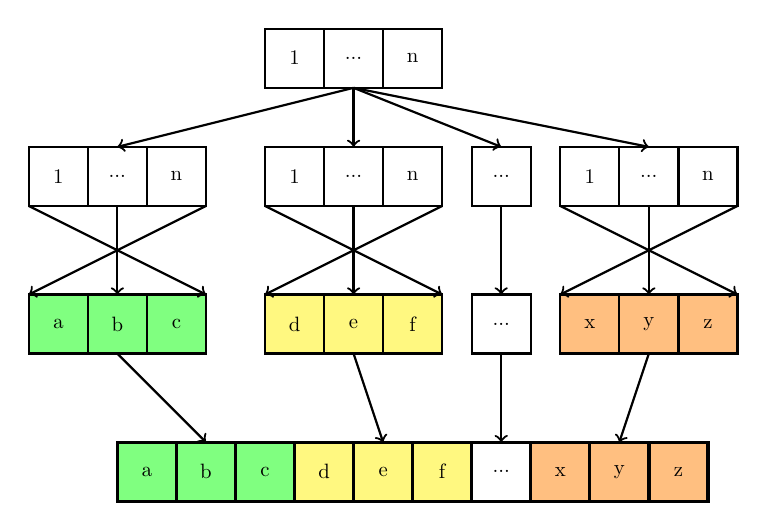
\begin{tikzpicture}[scale=0.75, transform shape]
	\draw [thick] (1,6.5) rectangle(2,7.5) node[pos=.5]{1};
	\draw [thick] (2,6.5) rectangle(3,7.5) node[pos=.5]{...};
	\draw [thick] (3,6.5) rectangle(4,7.5)node[pos=.5]{n};
	
	\draw [thick] (-3,4.5) rectangle(-2,5.5)node[pos=.5] {1};
	\draw [thick] (-2,4.5) rectangle(-1,5.5)node[pos=.5] {...};
	\draw [thick] (-1,4.5) rectangle(0,5.5)node[pos=.5] {n};
	
	\draw [thick] (1,4.5) rectangle(2,5.5)node[pos=.5] {1};
	\draw [thick] (2,4.5) rectangle(3,5.5)node[pos=.5] {...};
	\draw [thick] (3,4.5) rectangle(4,5.5)node[pos=.5] {n};
	
	\draw [thick] (4.5,4.5) rectangle(5.5,5.5)node[pos=.5] {...};
	
	\draw [thick,] (6,4.5) rectangle(7,5.5)node[pos=.5] {1};
	\draw [thick] (7,4.5) rectangle(8,5.5)node[pos=.5] {...};
	\draw [thick] (8,4.5) rectangle(9,5.5)node[pos=.5] {n};
	
	
	\draw [thick, fill=green!50] (-3,2) rectangle(-2,3)node[pos=.5] {a};
	\draw [thick, fill=green!50] (-2,2) rectangle(-1,3)node[pos=.5] {b};
	\draw [thick, fill=green!50] (-1,2) rectangle(0,3)node[pos=.5] {c};
	
	\draw [thick, fill=yellow!50] (1,2) rectangle(2,3)node[pos=.5] {d};
	\draw [thick, fill=yellow!50] (2,2) rectangle(3,3)node[pos=.5] {e};
	\draw [thick, fill=yellow!50] (3,2) rectangle(4,3)node[pos=.5] {f};
	
	
	\draw [thick] (4.5,2) rectangle(5.5,3)node[pos=.5] {...};
	
	\draw [thick, fill=orange!50] (6,2) rectangle(7,3)node[pos=.5] {x};
	\draw [thick, fill=orange!50] (7,2) rectangle(8,3)node[pos=.5] {y};
	\draw [thick, fill=orange!50] (8,2) rectangle(9,3)node[pos=.5] {z};

	
	\draw [very thick, fill=green!50] (-1.5,-0.5) rectangle(-0.5,0.5)node[pos=.5] {a};
	\draw [very thick, fill=green!50] (-0.5,-0.5) rectangle(0.5,0.5)node[pos=.5] {b};
	\draw [ very thick, fill=green!50] (0.5,-0.5) rectangle(1.5,0.5)node[pos=.5] {c};
	\draw [ very thick, fill=yellow!50] (1.5,-0.5) rectangle(2.5,0.5)node[pos=.5] {d};
	\draw [very thick, fill=yellow!50] (2.5,-0.5) rectangle(3.5,0.5)node[pos=.5] {e};
	\draw [very thick, fill=yellow!50] (3.5,-0.5) rectangle(4.5,0.5)node[pos=.5] {f};
	\draw [ very thick] (4.5,-0.5) rectangle(5.5,0.5)node[pos=.5] {...};
	\draw [ very thick, fill=orange!50] (5.5,-0.5) rectangle(6.5,0.5)node[pos=.5] {x};
	\draw [ very thick, fill=orange!50] (6.5,-0.5) rectangle(7.5,0.5)node[pos=.5] {y};
	\draw [ very thick, fill=orange!50] (7.5,-0.5) rectangle(8.5,0.5)node[pos=.5] {z};
	
	\draw [thick,draw=black,->] (2.5,6.5) -- (-1.5,5.5);
	\draw [thick,draw=black,->] (2.5,6.5) -- (2.5,5.5);
	\draw [thick,draw=black,->] (2.5,6.5) -- (5,5.5);
	\draw [thick,draw=black,->] (2.5,6.5) -- (7.5,5.5);
	
	\draw [thick,draw=black,->] (-3,4.5) -- (0,3);
	\draw [thick,draw=black,->] (-1.5,4.5) -- (-1.5,3);
	\draw [thick,draw=black,->] (0,4.5) -- (-3,3);
	
	\draw [thick,draw=black,->] (1,4.5) -- (4,3);
	\draw [thick,draw=black,->] (2.5,4.5) -- (2.5,3);
	\draw [thick,draw=black,->] (4,4.5) -- (1,3);
	
	\draw [thick,draw=black,->] (5,4.5) -- (5,3);
	
	\draw [thick,draw=black,->] (6,4.5) -- (9,3);
	\draw [thick,draw=black,->] (7.5,4.5) -- (7.5,3);
	\draw [thick,draw=black,->] (9,4.5) -- (6,3);
	
	\draw [thick,draw=black,->] (-1.5,2) -- (0,0.5);
	\draw [thick,draw=black,->] (2.5,2) -- (3,0.5);
	\draw [thick,draw=black,->] (5,2) -- (5,0.5);
	\draw [thick,draw=black,->] (7.5,2) -- (7,0.5);
	

	\end{tikzpicture}
	\caption[3.Optimierungsschritt]{Darstellung des dritten Optimierungsschritts. Hier werden die einzelnen Schritte des Ausgangsarray bis zum sortierten Array dargestellt.Der Master fügt die sortieren Teilarrays am Ende zusammen.}
	\label{fig:Ooptimierung}
\end{figure}

%Mögliche Optimierung (wenn nicht gewünscht weglassen)
\subsection{Optimierter Algorithmus}
Zusätzlich zu den Optimierungen am bestehenden Algorithmus wird eine alternative Aufteilung und Sortierung der Daten erarbeitet. Anstatt den initial Vektor auf einer Master Node auf eine unbestimmte Anzahl Worker aufzuteilen, kann eine Baumstruktur erstellt werden. Dabei sendet eine Ursprungsnode die Hälfte des Datensatzes an eine weitere Node. Diesen Prozess setzt jede Node unabhängig fort, bis alle Worker verwendet werden. Nun führt jeder Worker den Merge-Sort durch und sendet den sortierten Vektor wieder an die Node, von welcher er den Vektor erhalten hat. Diese Node führt nun durch die bestehende Funktion des Merge-Sorts die beiden sortierten Vektoren in einen sortierten Vektor zusammen und sendet diesen wiederum an die Node, von welcher die unsortierten Daten gesendet wurden. Dieser Prozess wird so lange wiederholt, bis die Ursprungsnode wieder die gesamten Daten hat. Das Ergebnis ist ein sortierter Vektor. Es werden hierbei nicht nur die Sortierungen Parallelisiert, sondern auch das Versenden der Daten, sowie das Zusammenführen der Daten. Die gleichzeitige Ausführung von mehreren Prozessen sorgt dabei für eine bessere Ausnutzung der verfügbaren Rechenkapazität. Aufgrund von mangelnder Zeit wurde dieser Algorithmus im Rahmen dieser Arbeit nicht implementiert und getestet.
\begin{figure}[!t]
	\centering
	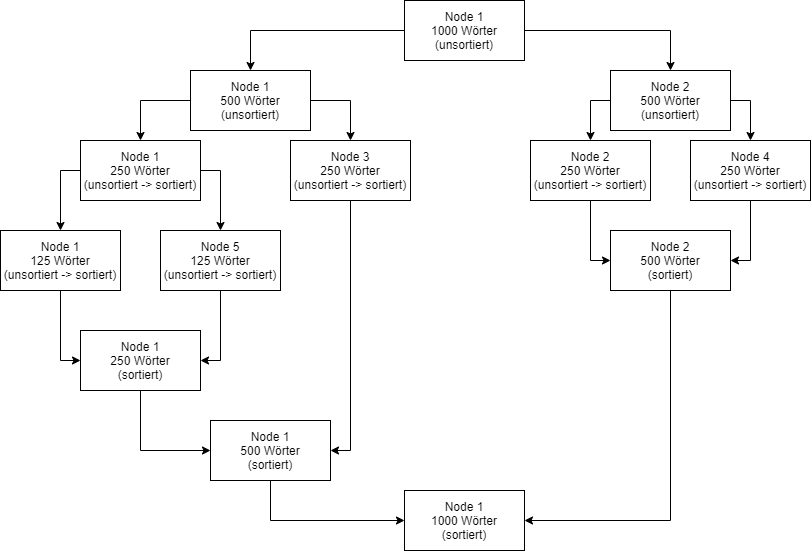
\includegraphics[width=3.5in]{Parallelisierungs_Algorithmus_2.png}
	\caption{Beispielhafter Durchlauf des Algorithmus mit 5 Nodes}
	\label{para_algo2}
\end{figure}
Grundsätzlich versprechen sich die Autoren von richtig implementierter Parallelisierung einen messbaren Zusammenhang von der Anzahl der verwendeten Rechenknoten und der resultierenden Laufzeit.
Um diese These zu überprüfen, und weitere mögliche Zusammenhänge zu erfassen, wurden im Rahmen der Arbeit umfassende Laufzeitmessungen durchgeführt.
Um Vergleichbarkeit herzustellen, wurden alle Messungen innerhalb kürzester Zeit am gleichen Tag vorgenommen. Aufgrund beschränkter Zeit wurde eine Stichprobengröße von $n = 10$ Messungen pro Messklasse gewählt.
Es sei angemerkt: wünschenswert und für eine statistisch fundierter Aussage notwendig wäre das fünf bis zehnfache hiervon. \paragraph
Die Messklassen werden hier über die Anzahl der verwendeten Rechenknoten festgelegt; für die Auswertung wurden Messungen mit einem bis sieben Rechenknoten durchgeführt.
Gemessen wird jeweils die benötigte Laufzeit, eine wohldefinierte und unveränderliche Datei bestehend aus einer großen Zahl von Wörtern zu sortieren.
Eine Messergebnis ist die mithilfe der Standard Template Bibliothek std::chrono gemessene Zeit, welche im Programmablauf des Master-Knotens zwischen dem Zeitpunkt unmittelbar vor der Verteilung der Teilelemente 
des zu sortierenden Textes an die Slave-Knoten und dem Zeitpunkt unmittelbar nach dem Zusammenführen der Ergebnisse der Slave-Rechenknoten verstreicht.
Das arithmetische Mittel sowie die Standardabweichung der Messreihen sind in Tabelle 1 aufgeführt.

\begin{table}
    \centering
    \caption{Zeitmessungen mit verschiedenen Anzahlen an Rechenknoten}
    \label{zeiten_tabelle}
    \begin{tabular}{l|lllllll}
    \textbf{Anzahl der Rechenknoten}  & \textbf{1} & \textbf{2} & \textbf{3} & \textbf{4} & \textbf{5} & \textbf{6} & \textbf{7}  \\ 
    \hline\hline
    \%\textbackslash{}bar\{t\}\$ [ms] & 4382.9     & 2413.7     & 2148.5     & 1728.6     & 1715.9     & 1621.6     & 1574.6      \\
    \$\textbackslash{}sigma\$ [ms]    & 491.2      & 128.0      & 113.9      & 72.2       & 70.9       & 62.3       & 112.4      
    \end{tabular}
\end{table}

Bei der Messreihe mit genau einem Rechenknoten ist eine erhöhte Unsicherheit zu erkennen. Dennoch ist der Mittelwert signifikant höher als bei allen anderen 
Messungen mit einer Rechenknotenanzahl größer eins. Bei den Anzahlen vier, fünf und sechs ist eine im Vergleich geringe Abweichung festzustellen. Diese Werte haben eine entsprechend hohe 
Aussagekraft. Interessanterweise sind die Mittelwerte der Zeiten ab einer Rechenknotenanzahl von 4 sehr nah beieinander. Daher kann mit den vorliegenden Daten keine statistisch begründete Aussage getroffen werden, ob sich die Rechenzeit ab einer Knotenzahl von 4 noch messbar verändert. Hierfür liegen die Messungen zu nah beieinander. Der scheinbar deutlich niedrigere Mittelwert der 7. Messung wird durch eine
höhere Messunsicherheit relativiert.

\paragraph

Eine umfassendere Darstellung der Daten erfolgt mithilfe eines Whiskers Plots, auch Kastenschaubild genannt (Abbildung X). Auch hier ist die vermutete, anfängliche und deutliche 
Absenkung der Laufzeiten über die Anzahl der Rechenknoten zu erkennen. Ebenfalls fällt ein starker Ausreißer bei der Knotenzahl eins auf. Auch bei Knotenzahlen zwei, vier und sechs 
gibt es solche Ausreißer. Interessanterweise gibt es gerade bei den Knotenzahlen vier und sechs, welche eine relativ geringe Standardabweichung aufweisen, ebenfalls Ausreißer nach oben. 
Im Kontext der niedrigen Standardabweichung bedeutet das einerseits, dass die restlichen Messwerte dieser Messreihen besonders konsistent sind. Andererseits könnte dies ein Hinweis darauf sein, dass die gemessenen Zeiten durch Zufall besonders konsistent und niedrig ausgefallen sind.

\begin{figure}[!t]
    \centering
    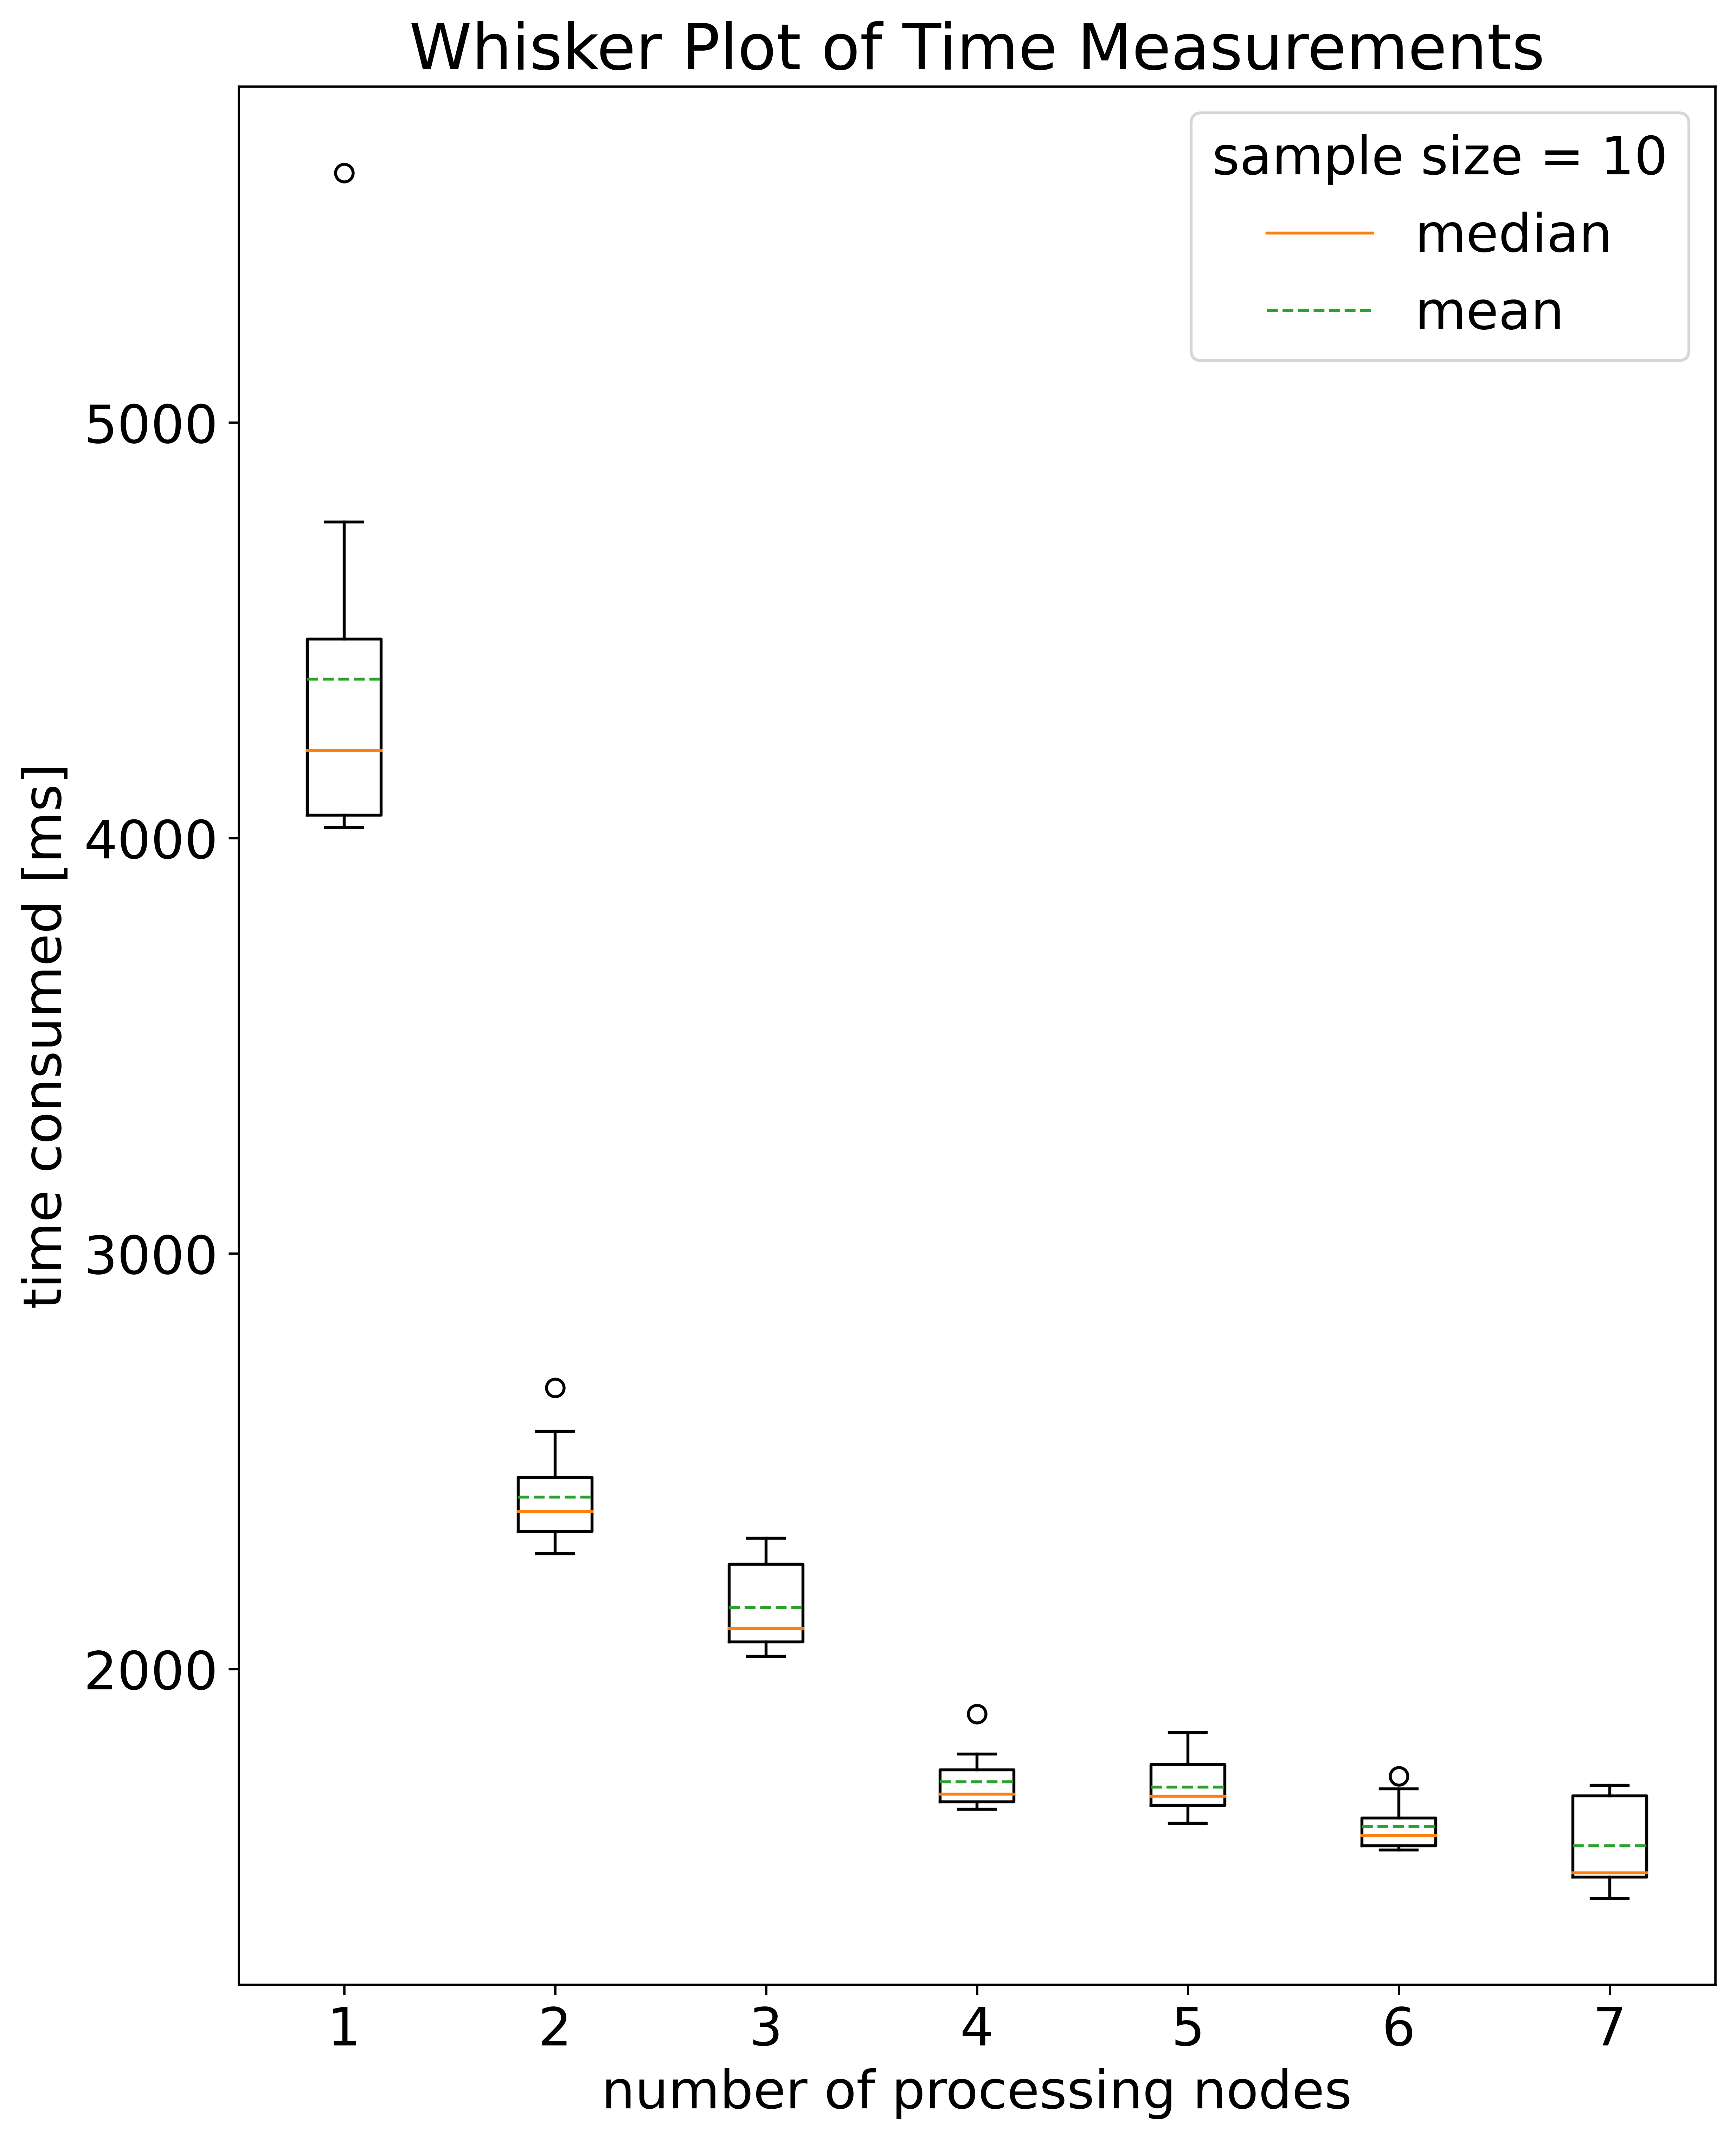
\includegraphics[width=8in]{boxplots.png}
    \caption{Cpation is already in picture!}
    \label{boxplot_times}
\end{figure}

\paragraph

So lassen die beobachteten Phänomene insgesamt darauf schließen, dass die Parallelisierung in ihrer für das Projekt durchgeführten Implementierung eine signifikante Absenkung der Laufzeit von bis zu einer Größenordnung von 60\% mit sich bringt. Dieser Effekt ist jedoch stark begrenzt und flacht mit einer steigenden Rechenknotenanzahl schnell ab bzw. verschwindet gänzlich. Die Effizienz pro Rechenknoten nimmt damit bei steigender Anzahl von Rechenknoten schnell ab.
Für genauere Aussagen ist eine größere Anzahl an Messungen pro Messklasse für nötig.

\paragraph

Eine Deutung für die Beobachteten Ergebnisse: die Rechenknoten in der Cloud sind mittels Ethernet miteinander verbunden, was das Senden und Empfangen von Nachrichten erstens nicht zeitlich deterministisch und zweitens anfällig für unregelmäßige und längere Laufzeiten macht. Offenbar bewegt sich bei der betrachteten Dateigröße das Senden und Empfangen von Nachrichten an mehr Knoten ab einer Knotenzahl von ca. vier in einer ähnlichen Größenordnungen wie der Laufzeitgewinn, welcher dadurch entsteht, dass ein Rechenknoten nur eine geringere Anzahl an Arbeit (Wörter sortieren) hat. Die Autoren vermuten, dass bei einer deutlich größeren Datei (mit mehr Wörtern), ein Laufzeitgewinn auch bei größeren Knotenzahlen zu messen sein wird.

\section{Fazit}
%\label{section:Fazit}
Durch den Vergleich zwischen der Laufzeit des Merge-Sort-Algorithmen ohne MPI mit dem parallelisierten Merge-Sort-Algorithmen werden Erkenntnisse gesammelt. Die Frage, die sich stellt: Bietet eine Parallelisierung mit MPI deutlich mehr Vorteile bei einem Merge-Sort-Algorithmus?\\

Bei der ersten Implementation benötigt der Merge-Sort der eingelesenen Datei von der Laufzeit länger. Erst ab fünf Prozessen ist MPI bei der Implementierung gleich schnell.
Bei der Gesamtlaufzeit ist die Laufzeit der Programmierung der Sende- und Empfangsvorgängen relevant. Die Zeit für die Sortierung nimmt einen geringen Anteil der Gesamtlaufzeit ein.
Da die Ausgangsimplementierung die Chars der Wörter einzeln versendet, erzielt eine Optimierung mit weniger Sende- und Empfangsvorgänge eine deutlich verbesserte Laufzeit. Durch diese Optimierung der ersten Implementation sind zwei Prozesse deutlich schneller als die Ausgangssituation ohne MPI. \\
Anhand der Laufzeit Messung ist ein graphischer Verlauf einer Exponentialverteilung zu erkennen, was darauf schließen lässt, dass bei einer gewissen Anzahl an Prozessen die Laufzeit nur minimal abweicht und bei vielen Prozessen eine Laufzeitverbesserung nicht mehr stattfindet.\\
Eine weitere Erkenntnis ist, dass die Laufzeit bei gleichbleibenden Prozessen und Wörtern keinen deterministischen Vorgang aufweist. Denn bei jedem neuen Aufruf des Merge-Sorts mit MPI variierte die Laufzeit. Dieses Ereignis tritt durch die Nutzung einer Cloud auf.\\

Zeitlich konnte der Optimierungsschritt III nicht mehr umgesetzt werden. Jedoch kann davon ausgegangen werden, dass die Laufzeit durch die beschriebene Optimierung \ref{Optimierung3} zusätzlich noch verbessert werden kann.

Anhand der Erkenntnisse und der Laufzeitauswertung ist zu sagen, dass MPI bei dem Merge-Sort-Algorithmus eine gute Performance bietet und die Laufzeit durch die Parallelisierung verkürzt. Das ist bei vielen Datenmengen mit umfangreichen Rechenanteil nützlich, damit die Prozesse parallel berechnet und die Ergebnisse am Ende zusammengeführt werden können.

\section*{Acknowledgment}

The preferred spelling of the word ``acknowledgment'' in America is without 
an ``e'' after the ``g''. Avoid the stilted expression ``one of us (R. B. 
G.) thanks $\ldots$''. Instead, try ``R. B. G. thanks$\ldots$''. Put sponsor 
acknowledgments in the unnumbered footnote on the first page.


\begin{thebibliography}{00}
\bibitem{b1} Dietmar Fey \glqq Grid-Computing: Eine Basistechnologie für Computational Science\grqq{}, Springer Verlag Heidelberg, Berlin, Seite 99-117 ,2010
\end{thebibliography}

\end{document}
